\documentclass[titlepage]{scrartcl}
\usepackage[ngerman]{babel}
\usepackage[T1]{fontenc}
\usepackage[utf8]{inputenc}
\usepackage{graphics}
\usepackage{graphicx}
\usepackage{tikz}
\usetikzlibrary{shapes.misc}

\tikzset{cross/.style={cross out, draw=black, minimum size=2*(#1-\pgflinewidth), inner sep=0pt, outer sep=0pt},cross/.default={2pt}}

\titlehead{Wintersemester 2023/24}
\title{\TicTacToe}
\subtitle{Product Backlog}
\date{Stand: \today}
\author{Jonas, Luis, Leonid}

\newcommand{\TicTacToe}{TI\reflectbox K Tac Toe}

\begin{document}
\maketitle

% Für welche Altersstufe ist die Software gedacht?
% Was soll bei den Schülern hängen bleiben?
	% Der Schüler soll erkennen können, dass die KI ein Gedächtnis hat und nach Häufigkeit des Gewinns aussucht.
% Bessere Beschreibung des Spiels im Produktziel (Interaktion, Zielgruppe)
% Kriterien weniger direkt fromulieren. (Abstrakter)
% Wie werden Kinder in der Gui angezeigt? Mit Symmetrie oder ohne?
% Umschalten: Wahrscheinlichkeiten oder Gewichte
% Funktionalitäten die nicht implementiert werden können, zu Annika weiterleiten.
% Release erstellen
% npm run test muss laufen
% Entwurfsdokumente auf dem neusten Stand halten in DoD

\emph{Hinweis:} Aufgrund der besseren Lesbarkeit ist in diesem Dokument nur von Spielern und Nutzern die Rede.
Es sind aber immer Spielerinnen und Spieler und Nutzerinnen und Nutzer aller Geschlechter gemeint.

"`Spieler"' meint im Folgenden immer die Entität, die eine der beiden Positionen im Spiel Tic-Tac-Toe (Kreuz oder Kreis) übernommen hat.
Die Person, die die App benutzt, wird "`Nutzer"' genannt.

\section{Produkt-Ziel}%schriftlicher Pitch der Software
Künstliche Intelligenz, insbesondere künstliche neuronale Netze, sind eines der Hot Topics in der Informatik.
Auch wenn das Thema im Bildungsplan Informatik in Baden-Württemberg bisher keinen Platz hat, kann nicht bezweifelt werden, dass es bei der nächsten Überarbeitung eingegliedert wird.
Andere Bundesländer sind hier teilweise weiter: Beispielsweise in Bayern ist "`Künstliche Intelligenz"' der größte der fünf Lernbereiche in Klasse 11, welcher auch in Klasse 13 wieder aufgenommen wird.

Die App "`\TicTacToe"' soll einen Beitrag für den sanften Einstieg in das Thema KI leisten.
Schülerinnen und Schüler können mit wenigen Klicks ein regelbasiertes Expertensystem erkunden, das nach und nach das Spiel "`Tic Tac Toe"' erlernt.
Dabei können die Schülerinnen und Schüler die Entscheidungen des Expertensystems schrittweise nachvollziehen und nehmen durch die Auswahl einer Belohnungsstrategie selbst Einfluss auf das Lernverhalten des Systems.
Sie lernen in diesem einfachen Setting das Konzept eines Brute-Force-Ansatzes sowie der Fehlerrückführung.

Die geplanten Funktionalitäten erlauben einen Einsatz im Unterricht nach einer Heranführung durch die Lehrkraft.
Wir gehen davon aus, dass den SuS die Hexapawn-Variante HER bereits bekannt ist.
Im Webinterface von "`\TicTacToe"' können die SuS den Entscheidungsbaum der KI erkunden, selbst gegen sie spielen oder zwei KIs gegeneinander trainieren lassen.
Am Ende einer Lerneinheit haben die SuS das Konzept von Gewichtsfunktionen nachvollzogen und können diese als "`Gedächtnis"' des Systems benennen, welches den Lernprozess abbildet.

\section{Didaktische Überlegungen}
Dieses Projekt und das Produkt "`\TicTacToe"' sind für den Informatikunterricht oder Informatik-AGs in der 7. bis 9. Klasse gedacht.
Sie soll jedoch auch für interessierte Schülerinnen und Schüler der Oberstufe spannend und informativ sein.
Eine Lerneinheit mit diesem Tool ist darauf ausgelegt immer von einer Lehrkraft begleitet zu werden und ist nicht komplett ohne Anleitung nützlich.
Schüler, die sich mit dem Tool beschäftigen, sollen nach Abschluss Lerneinheit nennen können, wie eine KI mit Hilfe von Gewichten lernen und trainiert werden kann.
Außerdem sollen sie auch in der Lage sein den Gewichte-Graphen als Gedächtnis der KI zu benennen und die Entscheidungen anhand dieses Graphen nachvollziehen zu können.
Ältere und schnellere Schüler können weiterhin beobachten und benennen,
wie sich unterschiedliche Belohnungsstrategien auf das Lernverhalten der KI auswirken und können diese aufgrund ihrer Beobachtungen auch bewerten.

%Erklären warum unsere Software cool ist (Stichwort: Einsatz)
\section{Funktionalitäten}% Kriterien: (vollständige) Definition der Software
\subsection{Muss-Kriterien}
	%Block1
	\begin{itemize}
		\item[M100] Während des Spiels wird ein 3x3-Tic-Tac-Toe-Spielfeld angezeigt.
		\item[M200] Die Felder des Spielfeldes können genau nach den Regeln von Tic-Tac-Toe besetzt werden.
		\item[M300] Die vorherigen Konfigurationen des Spielfeldes werden gespeichert und in einem Baum visualisiert.
		\item[M400] Alle Spielbrett-Konfigurationen, welche auf die momentane folgen können, können angezeigt werden (bis auf äquivalente Situationen).
		\item[M500] Eine einfache KI wählt auf Basis von Gewichten einen Zug aus.
		\item[M600] Um die KI zu trainieren werden durch Belohnungsstrategien die Gewichte der Pfade verändert.
		\item[M610] Es gibt mindestens eine Belohnungsstrategie.
		\item[M700] Der Nutzer kann die gegen die KI Tic-Tac-Toe spielen.
	\end{itemize}


\subsection{Soll-Kriterien}
	\begin{itemize}
		\item[S100] Automatisches Ziehen der KI kann an- und abgewählt werden.
		\item[S110] Ist das automatische Ziehen deaktiviert, so gibt es die Möglichkeit einzelne Züge der KI auszulösen.
		\item[S200] Es gibt die Möglichkeit, zwei KIs als Spieler auszuwählen.
		\item[S300] Die Zuggeschwindigkeit der KI kann festgelegt werden. %Frage: Wie didaktisch sinnvoll ist das gegen schnell vs langsam?
		\item[S400] Der Nutzer kann einstellen, dass nach Beenden eines Spiels automatisch das nächste Spiel mit den gleichen Einstellungen gestartet wird.
		\item[S500] Zwischen zwei Spielen besteht die Möglichkeit, die Gewichte der trainierte(n) KI(s) einzeln zurückzusetzen.
		\item[S600] Es gibt eine Ansicht, in der am Ende des Spiels die Belohnungsstrategie vom Nutzer angepasst werden kann.
		\item[S610] Eine Belohnungsstrategie ist die Elimination des letzten Zuges bei Verlust des Spiels.
		\item[S620] Eine Belohnungsstrategie ist Fehlerrückführung.
				Für Gewinnen, Unentschieden und Verlust werden die Gewichte der ausgeführten Züge individuell angepasst.
		\item[S630] Der Nutzer kann auswählen, dass die konfigurierte Belohnungsstrategie in Zukunft automatisch angewendet wird.
		\item[S700] Während der Auswahl der Belohnungsstrategie wird der Gewichte-Graph angezeigt. %Frage: Weiteres Scaffolding notwendig? Schüler haben bis jetzt nur den aktuellen Ablauf des Spiels gesehen nie den gesamten Graphen.
		\item[S710] Der Spielverlauf wird im Gewichte-Graph hervorgehoben.
	\end{itemize}

\subsection{Kann-Kriterien}
	\begin{itemize}
		\item[K100] Bei der Belohnungsstrategie Fehlerrückführung ist eine Aufschlüsselung der Belohnungen nach Spielstadium möglich.
				Das heißt, dass die Gewichte in der frühen Phase des Spiels anders angepasst werden können als die in der späteren Phase.
		\item[K110] Bei der Konfiguration der Belohnungsstrategie kann der Nutzer auswählen, dass die KI auch die Gewichte der Züge des Gegners anpasst. %Frage: Zu kompliziert für Zielgruppe?
		\item[K200] Die bisher ausgeführten Züge können rückgängig gemacht werden.
		\item[K300] Es ist eine Ansicht aufrufbar, in der der gesamte Gewichte-Graph angezeigt wird.
		\item[K400] Es ist eine perfekt spielende KI implementiert.
				Bei Start des Spiels kann diese fehlerlose KI anstelle des Nutzers oder einer anderen KI ausgewählt werden.
		\item[K500] Es gibt zu jedem Zeitpunkt die Möglichkeit, das aktuelle Spiel abzubrechen.
				Dabei werden die Gewichte der aktuell trainierten KI nicht geändert.
		\item[K600] Es gibt, solange das Spiel still steht, die Möglichkeit, die aktuell trainierte(n) KI(s) zu exportieren.
				Solange das Spiel still steht können Gewichte importiert werden, die dann die aktuellen Gewichte der ausgewählten KI überschreiben.
		\item[K700] Der Nutzer kann einstellen, dass nach Beenden eines Spiels die Start-Reihenfolge der Spieler automatisch getauscht wird.
		\item[K800] Statt Tic-Tac-Toe kann auch ein einfaches Brettspiel gespielt werden, für das die KI mit einer ähnlichen Entscheidungsbaum-Struktur trainiert wird. %einfaches --> anderes?


	\end{itemize}

	
\subsection{Abgrenzungskriterien}
	\begin{itemize}
		\item[A100] Die Gewichte der KI können nur über vorgegebene Belohnungsstrategien angepasst werden.
		\item[A200] Die Entscheidungen der KI basieren nur auf der aktuellen Spielsituation, nicht auf dem Spielverlauf.
	\end{itemize}
	
\section{Definition of Done}%Checkliste zur Überprüfung, ob ein Increment fertig ist
Ein Increment besteht aus einem oder mehreren Features.
Jedes Feature wird immer auf einem geeignetem \texttt{feature}-Branch implementiert.
Falls folgende Eigenschaften auf unser Projekt zutreffen, erklären wir das Feature für abgeschlossen:
\begin{itemize}
	\item Wichtige Funktionalitäten des Features sind mit UnitTests versehen.
	\item Der jeweilige Entwickler des Codes ist dafür verantwortlich auf seinem Branch einen Integrationstest durchzuführen.
	\item Eine relevante Änderung am produktiven Code wird nur in den \texttt{main}-Branch gemergt, wenn sie von einer zweiten Person gereviewt wurde.
			Ein Review wurde durchgeführt, sobald der Reviewer Fragen zum Code beantworten könnte und den Code für zufriedenstellend befunden hat.
			Der Reviewer ist dafür verantwortlich sicherzustellen, dass der \texttt{feature}-Branch auf aktuellem Stand ist und einen erneuten Integrationstest durchzuführen.
	\item Der Code des Features ist nach Review in den \texttt{main}-Branch gemergt.
	\item Unter Integrationstest verstehen wir, dass nach merge mit dem \texttt{main}-Branch der Kommandozeilen-Befehl \texttt{run test:unit} keine Fehlermeldungen ausgibt und der Kommandozeilen-Befehl \texttt{run dev} die Website mit den bereits implementierten Features erzeugt.
	\item Trello-Tickets des Features haben den Status "`Abgeschlossen"'.
\end{itemize}
Falls zusätzlich folgende Eigenschaften auf unser Projekt zutreffen, erklären wir das Increment für abgeschlossen:
\begin{itemize}
	\item Alle für das Increment geplanten Features wurden implementiert. Falls geplante Funktionalitäten nicht implementiert werden konnten, so wurde das mit den Product Ownern abgesprochen.
	\item Es wurde ein Release des aktuellen \texttt{main}-Branches erstellt.
	\item Der Kommandozeilen-Befehl \texttt{run test:unit} (Ausführen aller UnitTests) gibt keine Fehlermeldungen aus und der Kommandozeilen-Befehl \texttt{run dev} erzeugt die Website mit den bereits implementierten Features. %Frage: Muss hier npm run test:unit und npm run dev hin zur einfacheren Lesbarkeit für Ahnungslose?
\end{itemize}

\section{Definition of Fun}%Vereinbarungen über Zusammenarbeit
Wir vereinbaren die folgenden Regeln für unsere Zusammenarbeit:
\begin{itemize}
	\item Wir treffen uns vor jedem Dienstagstreffen 15 min vorher zur Koordination.
	\item Wir treffen uns jede Woche Freitags um 08:00 Uhr via Discord.
	\item Zu unseren Treffen kommen wir pünktlich und vorbereitet.
	\item Wenn wir auf Probleme stoßen (Implementierung, Setup, Zeitprobleme...), so kommunizieren wir diese offen und zeitnah.
	\item Wir dokumentieren unseren Fortschritt auf Trello.
	\item Wir behalten im Blick, dass neuer Code so früh abgeschlossen werden muss, dass ein Review noch vor der Abgabe möglich ist.
	\item Wir berichten im Discord über unseren Arbeitsfortschritt.
\end{itemize}

\section{Wichtige Entscheidungen}
\begin{itemize}
\item Ein 3x3-Spielbrett wird auf einer HTML und Javascript basierten Webseite angezeigt und auf diesem ist Tic-Tac-Toe spielbar.
\end{itemize}

\section{Offene Fragen}
\begin{itemize}
	\item Wo werden die Gewichte im Baum visualisiert? An den Kanten oder Knoten?
	\item Kann der gesamte Graph der Gewichte überhaupt sinnvoll und kompakt visualisiert werden?
\end{itemize}


\section{Projektplanung}%Verteilung der Scrum-Master-Tätigkeit
\begin{tabular}{lcc}
	Sprint &Thema& Scrum-Master\\
	0&Anforderung&--\\
	1&Entwurf & Luis\\
	2&Quali-sicherung & Jonas \\
	3&Abschluss & Leonid\\
\end{tabular}


\section{Epic}
%Epic über die Benutzung des TicTacToeamprojekts:

Ein Schüler öffnet die Website zum ersten Mal und sieht den Startbildschirm.
Auf diesem kann für Spieler 1 (Sp1) und Spieler 2 (Sp2) ausgewählt werden kann, ob eine KI oder der Schüler die Züge übernimmt.
Der Schüler wählt aus, dass er selbst (Sp1) gegen eine KI (Sp2) spielt und startet das Spiel per Knopfdruck.
Er setzt den ersten Stein auf ein Feld seiner Wahl und schaut sich an der Seite alle möglichen nächsten Züge von Sp2 an.
Er drückt auf einen Knopf, damit die KI für Sp2 zieht.
Nach seinem nächsten Zug wählt er aus, dass die KI die Züge ab jetzt automatisch spielt.
Im Folgenden macht die KI ihre Züge jetzt sobald der Schüler für Sp1 gezogen hat.
Nachdem das Spiel fertig gespielt ist wählt er die Belohnungsstrategie aus.
Dadurch werden die Gewichte der KI entsprechend angepasst.
Dies kann der Schüler im angezeigten Gewichte-Graph nachvollziehen.

Dann startet er das Spiel per Knopfdruck neu, wodurch er wieder auf den Startbildschirm kommt.
Er entscheidet sich gegen die gleiche KI erneut zu spielen, um sie weiter zu trainieren.
Er schaltet ein, dass der Startbildschirm nicht wieder angezeigt wird.
Da er auch mit dem Belohnungsalgorithmus zufrieden ist stellt er auch ein, dass der Belohnungsbildschirm nicht mehr angezeigt wird und erhöht die Geschwindigkeit, in der die KI einen Zug macht.

Im Folgenden spielt der Schüler gegen die KI mehrere Spiele, ohne dass der Startbildschirm oder der Belohnungsbildschirm angezeigt werden.
Die Gewichte der KI werden trotzdem nach jedem Spiel angepasst.

Nachdem er die KI nach seinen Wünschen trainiert hat, stellt er ein, dass er wieder in den Startbildschirm kommt.
Er löscht den Lernfortschritt der KI, um sie diesmal mit einem anderen Belohnungsalgorithmus zu trainieren.

\section{GUI-Entwurf}
\begin{figure}[ht]
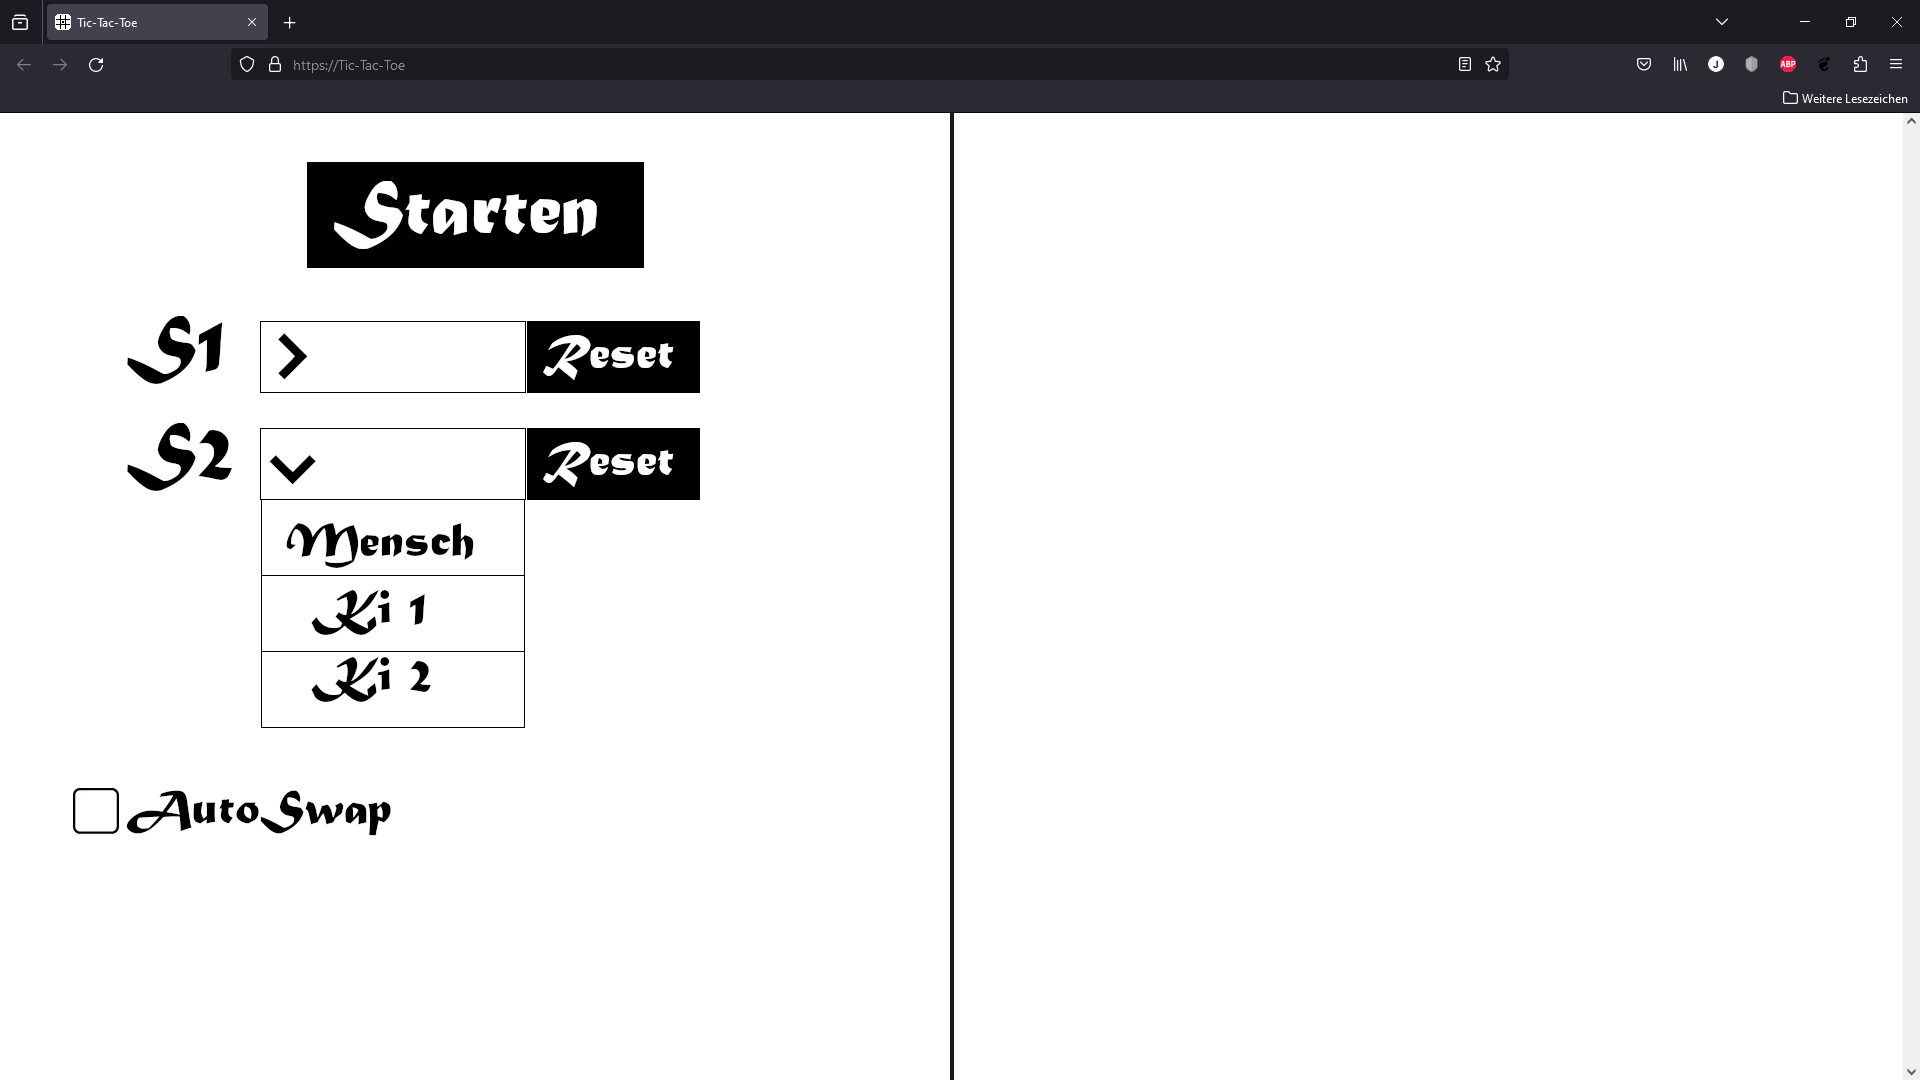
\includegraphics[width=\textwidth]{tictactoe_startansicht.png}
\caption{Ein erster Entwurf der Startansicht der Website, in welcher die Spielereinstellungen vorgenommen werden und ein Spiel gestartet werden kann.}
\end{figure}

\begin{figure}[ht]
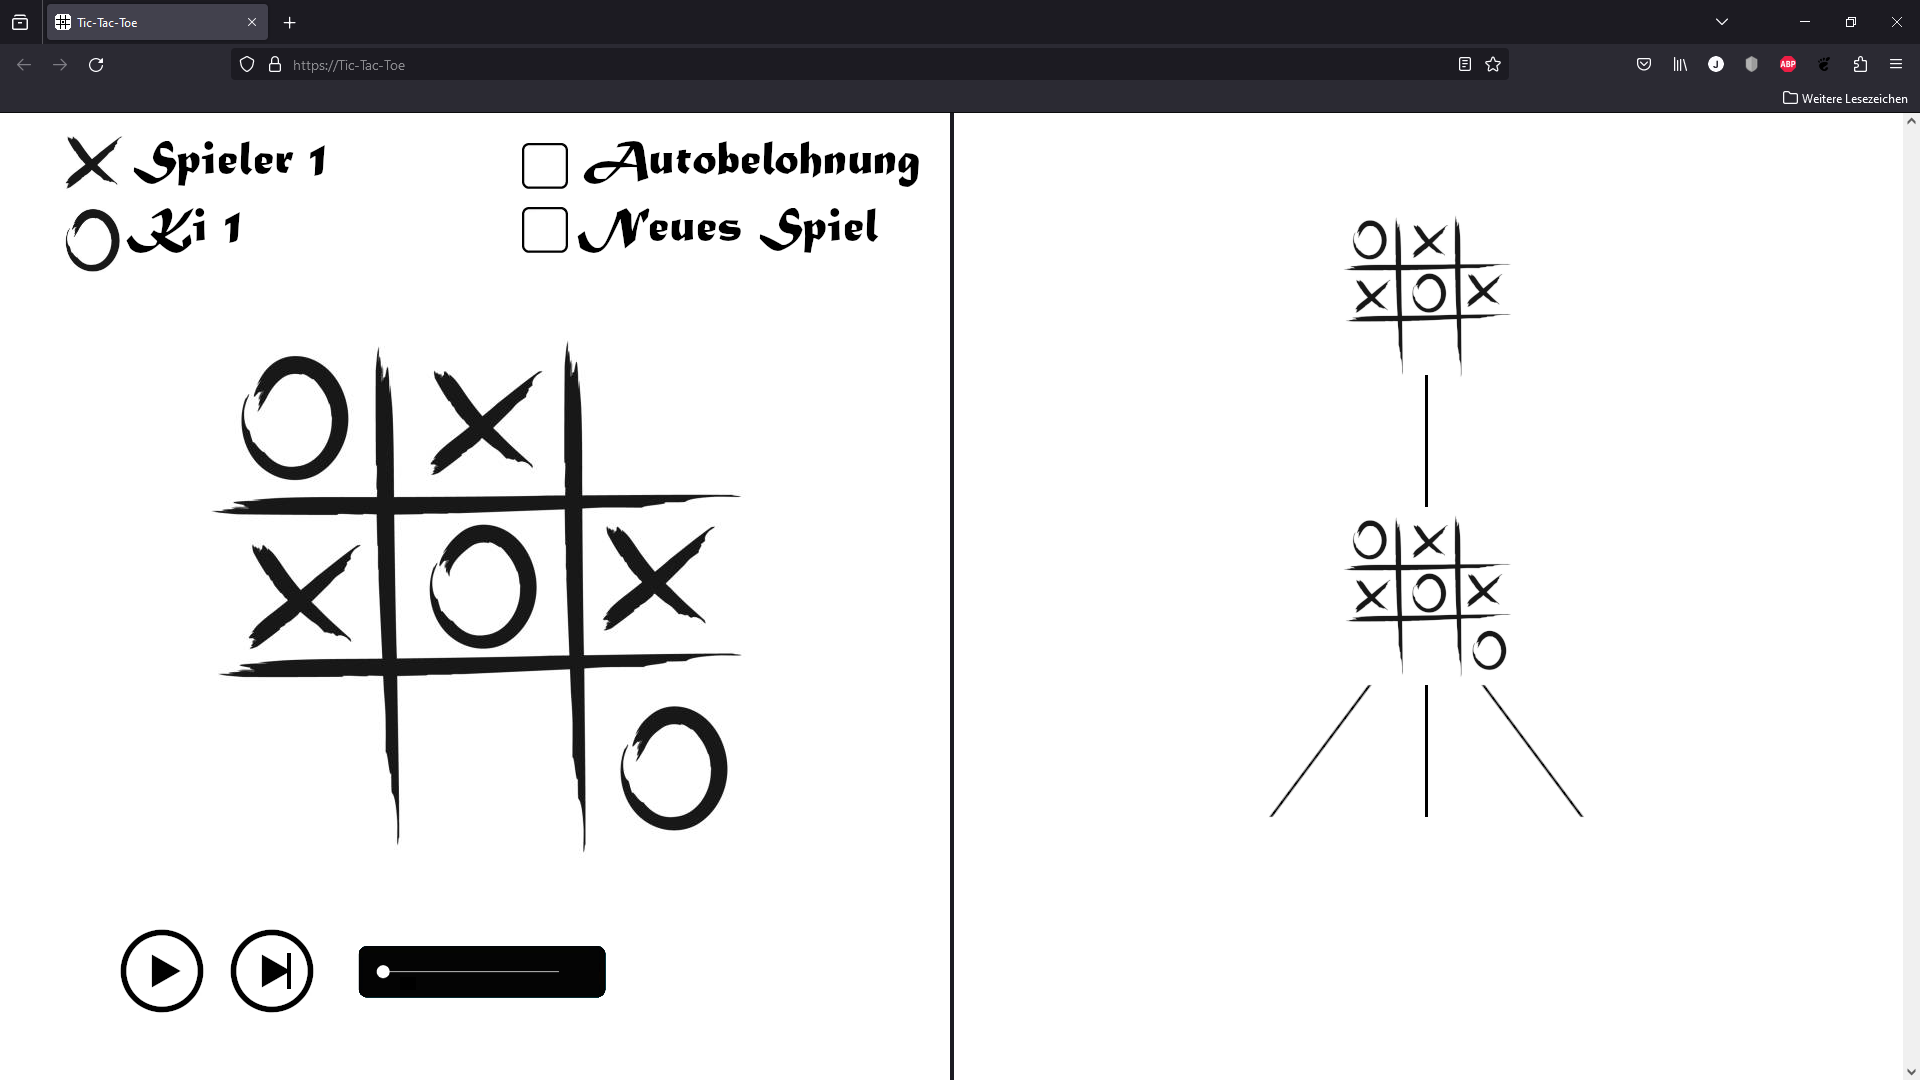
\includegraphics[width=\textwidth]{tictactoe_spielansicht.png}
\caption{Ein erster Entwurf der Spielansicht der Website, in welcher das Spiel Tic-Tac-Toe gespielt wird.}
\end{figure}

\begin{figure}[ht]
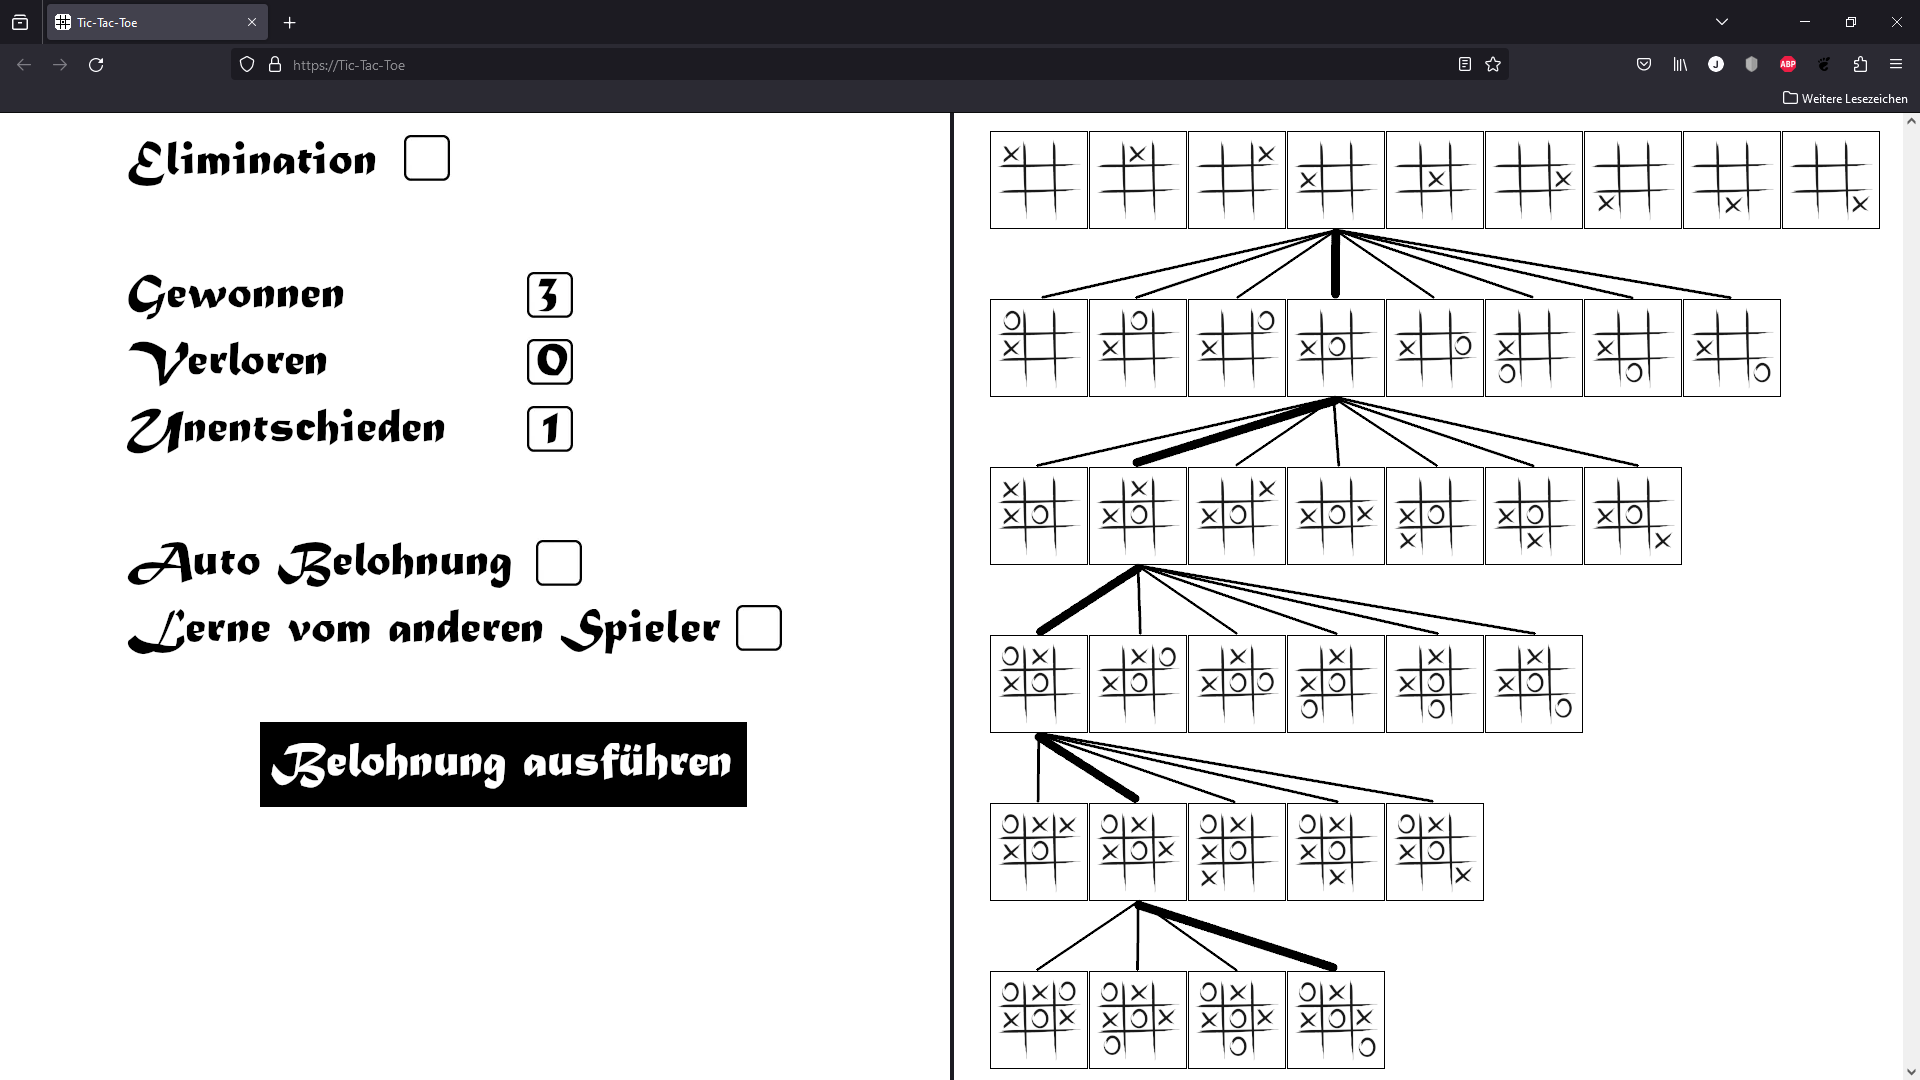
\includegraphics[width=\textwidth]{tictactoe_bewertungsansicht.png}
\caption{Ein erster Entwurf der Bewertungsansicht der Website, in welcher eingestellt wird, wie die Gewichtungen der KI nach einem Spiel anpasst werden.}
\end{figure}

\section{Burn-up-Chart}
\begin{figure}[ht]\centering
\begin{tikzpicture}[x=1cm, y=1cm]
	%Achsen
	\draw[->] (0,0) -- (9.5,0);
	\draw[->] (0,0) -- (0,8);
	\draw (-1,7.5) node[]{Aufwand};
	\draw (9,-1) node[]{Zeit};
	%Ticks
	\draw (3,0) ++(0,-0.1) --node[below]{\(1\)} ++(0,.2);
	\draw (6,0) ++(0,-0.1) --node[below]{\(2\)} ++(0,.2);
	\draw (9,0) ++(0,-0.1) --node[below]{\(3\)} ++(0,.2);
		%Graph
	\draw[very thick] (0,0) -- (1,0);%
										% -- (2,?)							
															%
	%Ziele
	\draw(3,7) node[cross]{};
	\draw[dashed] (1,0) -- (2,5) -- (3,6);
\end{tikzpicture}
\end{figure}
\end{document}
